\documentclass[addpoints,11pt]{exam}

% Page configurations
\title{ME: MECHANICAL ENGINEERING}
\usepackage[a4paper,bottom=1in,top=1in]{geometry}
\usepackage{amsmath}
\usepackage{graphicx}
\usepackage{tikz}
\usetikzlibrary{arrows}
\usetikzlibrary{decorations.markings}
\graphicspath{{images/}}

\usepackage{xpatch}
\xpatchcmd{\oneparchoices}{\penalty -50\hskip 1em plus 1em\relax}{\hfill}{}{}

% Header and footer
\pagestyle{headandfoot}
\headrule
\header{2008}{}{MAIN PAPER - ME}
\footrule
\footer{ME}{}{\thepage/\numpages}

\renewcommand{\thequestion}{Q.\arabic{question}}
\renewcommand{\thechoice}{(\Alph{choice})}
\renewcommand{\choicelabel}{\thechoice}

\begin{document}
\begin{center}
    \Large
    \textbf{ME: MECHANICAL ENGINEERING}
\end{center}

\textit{Duration} : Three hours
\hfill
\textit{Maximum Marks} : 150
\\\\
\textbf{Read the following instructions carefully}
\begin{enumerate}
    \item This question paper contains \textbf{24} printed pages including pages for rough work. Please check all pages and report discrepancy, if any.
    \item Write your registration number, your name and name of the examination centre at the specified locations on the right half of the ORS.
    \item Using HB pencil, darken the appropriate bubble under each digit of your registration number and the letters corresponding to your paper code.
    \item All the questions in this question paper are of objective type.
    \item Questions must be answered on \textbf{O}bjective \textbf{R}esponse \textbf{S}heet (\textbf{ORS}) by darkening the appropriate bubble (marked A, B, C, D) using HB pencil against the question number on the left hand side of the ORS. \textbf{Each question has only one correct answer}. In case you wish to change an answer, erase the old answer completely. More than one answer bubbled against a question will be treated as a wrong answer.
    \item Questions 1 through 20 are 1-mark questions and questions 21 through 85 are 2-mark questions.
    \item Questions 71 through 73 is one set of common data questions. The question pairs (76, 77), (78, 79), (80, 81), (82, 83) and (84, 85) are questions with linked answers. The answer to the second question of the above pairs will depend on the answer to the first question of the pair. If the first question in the linked pair is wrongly answered or is un-attempted, then the answer to the second question will not be evaluated.
    \item Unattempted questions will carry zero marks.
    \item \textbf{NEGATIVE MARKING}: For Q.1 to Q.20, \textit{\textbf{0.25}} mark will be deducted for each wrong answer. For Q.21 to Q.75, \textit{\textbf{0.5}} mark will be deducted for each wrong answer. For the pairs of questions with linked answers, there will be negative marks only for wrong answer to the first question, i.e. for Q.76, Q.78, Q.80, Q.82 and Q.84, \textit{\textbf{0.5}} mark will be deducted for each wrong answer. There is no negative marking for Q.77, Q.79, Q.81, Q.83 and Q.85.
    \item Calculator \textbf{without data connectivity} is allowed in the examination hall.
    \item Charts, graph sheets and tables are NOT allowed in the examination hall.
    \item Rough work can be done on the question paper itself. Additional blank pages are given at the end of the question paper for rough work.
\end{enumerate}
\newpage

\large\textbf{Q.1 -- Q.20 carry one mark each.}\\
\begin{questions}

    \question In the Taylor series expansion of $e^x$ about x=2, the coefficient of $(x-2)^4$ is\\

    \begin{oneparchoices}
        \choice $\frac{1}{4!}$
        \choice $\frac{2^4}{4!}$
        \choice $\frac{e^2}{4!}$
        \choice $\frac{e^4}{4!}$
    \end{oneparchoices}\\

    \question Given that $\ddot{x} + 3x = 0$, and $x(0)=1$, $\dot{x}(0)=(0)$, what is $x(1)$?\\

    \begin{oneparchoices}
        \choice $-0.99$
        \choice $-0.16$
        \choice $0.16$
        \choice $0.99$
    \end{oneparchoices}\\

    \question The value of $\lim{x\rightarrow8} \frac{x^{\frac{1}{3}}-2}{(x-8)}$ is\\

    \begin{oneparchoices}
        \choice $\frac{1}{16}$
        \choice $\frac{1}{12}$
        \choice $\frac{1}{8}$
        \choice $\frac{1}{4}$
    \end{oneparchoices}\\

    \question A coin is tossed 4 times. What is the probability of getting heads exactly 3 times?\\

    \begin{oneparchoices}
        \choice $\frac{1}{4}$
        \choice $\frac{3}{8}$
        \choice $\frac{1}{2}$
        \choice $\frac{3}{4}$
    \end{oneparchoices}\\

    \question The matrix $\begin{bmatrix}
            1 & 2 & 4 \\
            3 & 0 & 6 \\
            1 & 1 & p
        \end{bmatrix}$ has one eigenvalue equal to 3. The sum of the other two eigenvalues is\\

    \begin{oneparchoices}
        \choice $p$
        \choice $p-1$
        \choice $p-2$
        \choice $p-3$
    \end{oneparchoices}\\

    \question The divergence of the vector field $(x-y)\hat{i} + (y-x)\hat{j} + (x+y+z)\hat{k}$ is\\

    \begin{oneparchoices}
        \choice $0$
        \choice $1$
        \choice $2$
        \choice $3$
    \end{oneparchoices}\\

    \question The transverse shear stress acting in a beam of rectangular cross-section, subjected to a transverse shear load, is\\

    \begin{choices}
        \choice variable with maximum at the bottom of the beam
        \choice variable with maximum at the top of the beam
        \choice uniform
        \choice variable with maximum on the neutral axis
    \end{choices}
\pagebreak

    \question A rod of length $L$ and diameter $D$ is subjected to a tensile load $P$. Which of the following is sufficient to calculate the resulting change in diameter?\\

    \begin{choices}
        \choice Young's modulus
        \choice Shear modulus
        \choice Poisson's ratio
        \choice Both Young's modulus and shear modulus
    \end{choices}

    \question A straight rod of length $L(t)$, hinged at one end and freely extensible at the other end, rotates through an angle $\theta(t)$ about the hinge. At time $t$, $L(t)=1$ m, $\dot{L}(t)=1$ m/s, $\theta(t)=\frac{\pi}{4}$rad and $\dot{\theta}(t)=1$ rad/s. The magnitude of the velocity at the other end of the rod is\\

    \begin{oneparchoices}
        \choice $1$m/s
        \choice $\sqrt{2}$m/s
        \choice $\sqrt{3}$m/s
        \choice $2$m/s
    \end{oneparchoices}\\

    \question A cantilever type gate hinged at Q is shown in the figure. P and R are the centers of gravity of the cantilever part and the counterweight respectively. The mass of the cantilever part is 75 kg. The mass of the coutnerweight, for static balance, is\\

    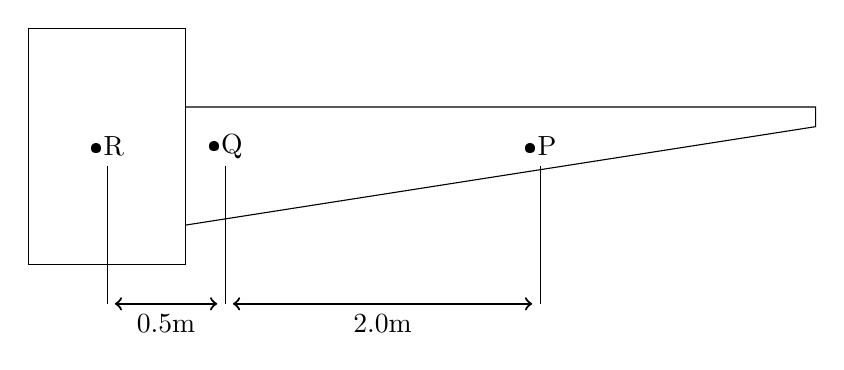
\begin{tikzpicture}
        \draw (0,0) rectangle (2,3);
        \node at (1,1.5) {•R};
        \draw[very thin] (1,1.25) -- (1,-0.5);
        \draw (2,2) -- (10,2) -- (10,1.75) -- (2,0.5);
        \node at (2.5,1.5) {•Q};
        \draw[very thin] (2.5,1.25) -- (2.5,-0.5);
        \node at (6.5,1.5) {•P};
        \draw[very thin] (6.5,1.25) -- (6.5,-0.5);
        \draw[thick, <->] (1.1,-0.5) -- (2.4,-0.5);
        \draw[thick, <->] (2.6,-0.5) -- (6.4,-0.5);
        \node at (1.75,-0.75) {0.5m};
        \node at (4.5,-0.75) {2.0m};
    \end{tikzpicture}

    \begin{oneparchoices}
        \choice 75kg
        \choice 150kg
        \choice 225kg
        \choice 300kg
    \end{oneparchoices}\\

    \question A planar mechanism has 8 links and 10 rotary joints. The number of degrees of freedom of the mechanism, using Greubler's criterion, is\\

    \begin{oneparchoices}
        \choice $0$
        \choice $1$
        \choice $2$
        \choice $3$
    \end{oneparchoices}\\

    \question An axial residual compressive stress due to a manufacturing process is present on the outer surface of a rotating shaft subjected to bending. Under a given bending load, the fatigue life of the shaft in the presence of residual compressive stress is\\

    \begin{choices}
        \choice decreased
        \choice increased or decreased, depending on the external bending load
        \choice neither decreased nor increased
        \choice increased
    \end{choices}

    \question 2 moles of oxygen are mixed adiabatically with another 2 moles of oxygen in a mixing chamber, so that the final total pressure and temperature of the mixture become same as those of the individual constituents at their intial states. The universal gas constant is given as $R$. The change in entropy due to mixing, per mole of oxygen, is given by\\

    \begin{oneparchoices}
        \choice $-R \ln2$
        \choice $0$
        \choice $R \ln 2$
        \choice $R\ln4$
    \end{oneparchoices}\\

    \question For flow of liquid over a heated plate, the following fluid properties are known:\\\\
    viscosity = 0.001 Pa.s ; specific heat constant pressure = 1kJ/kg.K ;\\
    thermal conductivity = 1 W/m.K.\\
    The hydrodynamic boundary layer thickness at a specified location on the plate is 1 mm. The thermal boundary layer thickness at the same location is

    \begin{oneparchoices}
        \choice 0.001 mm
        \choice 0.01 mm
        \choice 1 mm
        \choice 1000 mm
    \end{oneparchoices}\\

    \question For the continuity equation given by $\overrightarrow{\nabla}\cdot\overrightarrow{V} = 0$ to be valid, where $\bar{V}$ is the velocity vector, which one of the following is a necessary condition?\\

    \begin{choices}
        \choice steady flow
        \choice irrotational flow
        \choice inviscid flow
        \choice incompressible flow
    \end{choices}

    \question Which one of the following is NOT a necessary assumption for the air-standard Otto cycle?\\

    \begin{choices}
        \choice All processes are both internally as well as externally reversible.
        \choice Intake and exhaust processes are constant volume heat rejection processes.
        \choice The combustion process is a constant volume heat addition process.
        \choice The working fluid is an ideal gas with constant specific heats.
    \end{choices}

    \question In an M/M/1 queueing system, the number of arrivals in an interval of length $T$ is a Poisson random variable (i.e. the probability of there being $n$ arrivals in an interval of length $T$ is $\frac{e^{-\lambda T}(\lambda T)^n}{n!}$). The probability density function $f(t)$ of the inter-arrival time is given by\\

    \begin{oneparchoices}
        \choice $\lambda^2(e^{-\lambda^2t})$
        \choice $\frac{e^{-\lambda^2t}}{\lambda^2}$
        \choice $\lambda e^{-\lambda t}$
        \choice $\frac{e^{-\lambda t}}{\lambda}$
    \end{oneparchoices}\\

    \question A set of 5 jobs is to be processed on a single machine. The processing time (in days) is given in the table below. The holding cost for each job is Rs. $K$ per day.\\\\
    \begin{center}
        \begin{tabular}{|l|l|}
            \hline
            \textbf{Job} & \textbf{Processing time} \\
            \hline
            P            & 5                        \\\hline
            Q            & 2                        \\\hline
            R            & 3                        \\\hline
            S            & 2                        \\\hline
            T            & 1                        \\\hline
        \end{tabular}
    \end{center}
    A schedule that minimizes the total inventory cost is

    \begin{oneparchoices}
        \choice T-S-Q-R-P
        \choice P-R-S-Q-T\\
        \choice T-R-S-Q-P
        \choice P-Q-R-S-T
    \end{oneparchoices}\\

    \question For generating a Coon's surface we require\\
    \begin{choices}
        \choice a set of grid points on the surface
        \choice a set of grid control points
        \choice four bounding curves defining the surface
        \choice two bounding curves and a set of grid control points
    \end{choices}

    \question Internal gear cutting operation can be performed by\\
    \begin{choices}
        \choice milling
        \choice shaping with rack cutter
        \choice shaping with pinion cutter
        \choice hobbing
    \end{choices}
    \pagebreak
    \large\textbf{Q.21 -- Q.75 carry two marks each.}\\
    \question Consider the shaded triangular region $P$ shown in the figure. What is $\iint\limits_P xy\mathrm{d}x\mathrm{d}y$?\\
    \begin{center}
        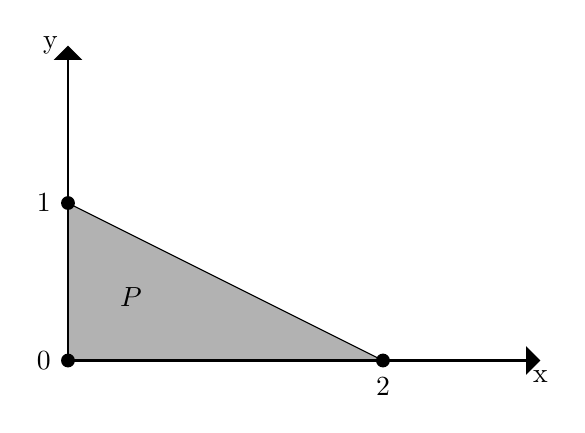
\begin{tikzpicture}[scale=2]
            \centering
            \fill[black!30!white] (0,0) -- (2,0) -- (0,1) -- cycle;
            \node at (0.4,0.4) {$P$};
            \draw (0,1) -- (2,0);
            \draw[thick,-triangle 90] (0,0) -- (3,0) node [below] {x};
            \draw[thick,-triangle 90] (0,0) -- (0,2) node [left] {y};
            \node[circle,fill=black,inner sep=0pt,minimum size=5pt,label=below:2] at (2,0) {};
            \node[circle,fill=black,inner sep=0pt,minimum size=5pt,label=left:0] at (0,0) {};
            \node[circle,fill=black,inner sep=0pt,minimum size=5pt,label=left:1] at (0,1) {};
        \end{tikzpicture}
    \end{center}

    \begin{oneparchoices}
        \choice $\frac{1}{6}$
        \choice $\frac{2}{9}$
        \choice $\frac{7}{2}$
        \choice $1$
    \end{oneparchoices}\\

    \question The directional derivative of the scalar function $f(x,y,z) = x^2 + 2y^2 + z$ at the point $P=(1,1,2)$ in the direction of vector $\overrightarrow{a} = 3\hat{i} -4\hat{j}$ is\\

    \begin{oneparchoices}
        \choice $-4$
        \choice $-2$
        \choice $-1$
        \choice $1$
    \end{oneparchoices}\\
    \question For what value of $a$, if any, will the following system of equations in $x$, $y$ and $z$ have a solution?\\\\
    $2x+3y=4$\\$x+y+z=4$\\$x+2y-z=a$

        \begin{oneparchoices}
            \choice Any real number
            \choice $0$
            \choice $1$
            \choice There is no such value
        \end{oneparchoices}\\
        \question Which of the following integrals is unbounded?\\

        \begin{oneparchoices}
            \choice $\int_{0}^{\pi/4}{\tan x dx}$
            \choice $\int_{0}^{\infty}{\frac{1}{x^2+1} dx}$
            \choice $\int_{0}^{\infty}{xe^{-x} dx}$
            \choice $\int_{0}^{1}{\frac{1}{1-x} dx}$
        \end{oneparchoices}\\

        \question The integral $\oint{f(z)dz}$ evaluated around the unit circle on the complex plane for $f(z) = \frac{\cos z}{z}$ is\\

        \begin{oneparchoices}
            \choice $2\pi i$
            \choice $4\pi i$
            \choice $-2\pi i$
            \choice $0$
        \end{oneparchoices}\\

        \question The length of the curve $y=\frac{2}{3}x^{\frac{3}{2}}$ from $x=0$ to $x=1$ is\\

        \begin{oneparchoices}
            \choice $0.27$
            \choice $0.67$
            \choice $1$
            \choice $1.22$
        \end{oneparchoices}\\

        \question The eigenvectors of the matrix $\begin{bmatrix}
        1 & 2 \\
        0 & 2
    \end{bmatrix}$ are written in the form $\begin{bmatrix}
        1 \\
        a
    \end{bmatrix}$ and $\begin{bmatrix}
        1 \\b
    \end{bmatrix}$. What is $a+b$?

        \begin{oneparchoices}
            \choice $0$
            \choice $\frac{1}{2}$
            \choice $1$
            \choice $2$
        \end{oneparchoices}\\

        \question Let $f = y^x$. What is $\frac{\partial^2 f}{\partial{x}\partial{y}}$ at $x=2$, $y=1$?\\

        \begin{oneparchoices}
            \choice $0$
            \choice $\ln 2$
            \choice $1$
            \choice $\frac{1}{\ln 2}$
        \end{oneparchoices}\\

        \question It is given that $y'' + 2y' + y=0$, $y(0)=0$, $y(1)=0$. What is $y(0.5)$?\\

        \begin{oneparchoices}
            \choice $0$
            \choice $0.37$
            \choice $0.62$
            \choice $1.13$
        \end{oneparchoices}\\

        \question The strain energy stored in the beam with flexural rigidity $EI$ and loaded as shown in the figure is\\

        \begin{center}
            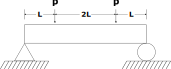
\includegraphics[scale=0.5]{q30}
        \end{center}

        \begin{oneparchoices}
            \choice $\frac{P^2L^3}{3EI}$
            \choice $\frac{2P^2L^3}{3EI}$
            \choice $\frac{4P^2L^3}{3EI}$
            \choice $\frac{8P^2L^3}{3EI}$
        \end{oneparchoices}\\

        \question For the component loaded with a force $F$ as shown in the figure, the axial stress at the corner point $P$ is\\

        \begin{center}
            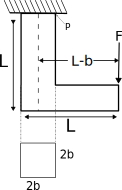
\includegraphics[scale=0.3]{q31}
        \end{center}

        \begin{oneparchoices}
            \choice $\frac{F(3L-b)}{4b^3}$
            \choice $\frac{F(3L+b)}{4b^3}$
            \choice $\frac{F(3L-4b)}{4b^3}$
            \choice $\frac{F(3L-2b)}{4b^3}$
        \end{oneparchoices}\\

        \question A solid circular shaft of diameter 100 mm is subjected to an axial stress of 50 MPa. It is further subjected to a torque of 10 kNm. The maximum principal stress experienced on the shaft is closest to\\

        \begin{oneparchoices}
            \choice 41 MPa
            \choice 82 MPa
            \choice 164 MPa
            \choice 204 MPa
        \end{oneparchoices}\\

        \question A circular disk of radius $R$ rolls without slipping at a velocity $v$. The magnitude of velocity at point $P$ (see figure) is: % TODO\\

        \begin{oneparchoices}
            \choice $\sqrt{3}v$
            \choice $\sqrt{3}v/2$
            \choice $v/2$
            \choice $2v/\sqrt{3}$
        \end{oneparchoices}\\

        \question Consider a truss PQR loaded at P with a force $F$ as shown in the figure. %TODO\\
        The tension in the member QR is

        \begin{oneparchoices}
            \choice 0.5 $F$
            \choice 0.63 $F$
            \choice 0.73 $F$
            \choice 0.87 $F$
        \end{oneparchoices}\\

        \question The natural frequency of the spring mass system shown in the figure is closest to %TODO\\

        \begin{oneparchoices}
            \choice 8 Hz
            \choice 10 Hz
            \choice 12 Hz
            \choice 14 Hz
        \end{oneparchoices}\\

        \question The rod PQ of length $L$ and with flexural rigidity $EI$ is hinged at both ends. For what minimum force $F$ is it expected to buckle?\\

        \begin{oneparchoices}
            \choice $\frac{\pi^2EI}{L^2}$
            \choice $\frac{\sqrt{2}\pi^2EI}{L^2}$
            \choice $\frac{\pi^2EI}{\sqrt{2}L^2}$
            \choice $\frac{\pi^2EI}{2L^2}$
        \end{oneparchoices}\\

        \question In a cam design, the rise motion is given by a simple harmonic motion (SHM) $s=\frac{h}{2}(1-\cos\frac{\pi\theta}{\beta})$, where $h$ is the total rise, $\theta$ is camshaft angle, $\beta$ is the total angle of the rise interval. The jerk is given by\\

        \begin{oneparchoices}
            \choice $\frac{h}{2}(1-\cos\frac{\pi\theta}{\beta})$
            \choice $\frac{\pi}{\beta}\frac{h}{2}\sin\frac{\pi\theta}{\beta}$
            \choice $\frac{\pi^2}{\beta^2}\frac{h}{2}\cos\frac{\pi\theta}{\beta}$
            \choice $-\frac{\pi^3}{\beta^3}\frac{h}{2}\sin\frac{\pi\theta}{\beta}$
        \end{oneparchoices}\\

        \question A uniform rigid rod of mass $m=1$ kg and length $L=1$ m is hinged at its centre and laterally supported at one end by a spring of spring constant $k=300$ N/m. The natural frequency $\omega_n$ in rad/s is\\

        \begin{oneparchoices}
            \choice 10
            \choice 20
            \choice 30
            \choice 40
        \end{oneparchoices}\\

        \question A compression spring is made of music wire of 2 mm diameter having a shear strength and shear modulus of 800 MPa and 80 GPa respectively. The mean coil diameter is 20 mm, free length is 40 mm and the number of active coils is 10. If the mean coil diameter is reduced to 10 mm, the stiffness of the spring is approximately\\

        \begin{oneparchoices}
            \choice decreased by 8 times
            \choice decreased by 2 times
            \choice increased by 2 times
            \choice increased by 8 times
        \end{oneparchoices}\\

        \question A journal bearing has a shaft diameter of 40 mm and a length of 40 mm. The shaft is rotating at 20 rad/s and the viscosity of lubricant is 20 mPa.s. The clearance is 0.020 mm. The loss of torque due to the viscosity of the lubricant is approximately.\\

        \begin{oneparchoices}
            \choice 0.040 Nm
            \choice 0.252 Nm
            \choice 0.400 Nm
            \choice 0.652 Nm
        \end{oneparchoices}\\

        \question A clutch has outer and inner diameters 100 mm and 40 mm respectively. Assuming a uniform pressure of 2 MPa and coefficient of friction of liner material 0.4, the torque carrying capacity of the clutch is\\

        \begin{oneparchoices}
            \choice 148 Nm
            \choice 196 Nm
            \choice 372 Nm
            \choice 490 Nm
        \end{oneparchoices}\\

        \question A spur gear has a module of 3 mm, number of teeth 16, a face width of 36 mm and a pressure angle of $20^\circ$. It is transmitting a power of 3 kW at 20 rev/s. Taking a velocity factor of 1.5, and a form factor of 0.3, the stress in the gear tooth is about\\

        \begin{oneparchoices}
            \choice 32 MPa
            \choice 46 MPa
            \choice 58 MPa
            \choice 70 MPa
        \end{oneparchoices}\\

        \question Match the type of gears with their most appropriate description.\\\\
        \begin{tabular}{|p{0.2in}|p{1in}|p{0.2in}|p{0.2in}|p{3in}|}
            \hline
              & Type of gear    &  &   & Description                                                                 \\
            \cline{1-2}\cline{4-5}
            P & Helical         &  & 1 & Axes non parallel and non intersecting                                      \\
            \cline{1-2}\cline{4-5}
            Q & Spiral Bevel    &  & 2 & Axes parallel teeth are inclined to the axis                                \\
            \cline{1-2}\cline{4-5}
            R & Hypoid          &  & 3 & Axes parallel teeth are parallel to the axis                                \\
            \cline{1-2}\cline{4-5}
            S & Rack and pinion &  & 4 & Axes are perpendicular and intersecting, and teeth are inclined to the axis \\
            \cline{1-2}\cline{4-5}
              &                 &  & 5 & Axes are perpendicular and used for large speed reduction                   \\
            \cline{1-2}\cline{4-5}
              &                 &  & 6 & Axes parallel and one of the gears has infinite radius                      \\
            \cline{1-2}\cline{4-5}
        \end{tabular}

        \begin{oneparchoices}
            \choice P-2, Q-4, R-1, S-6
            \choice P-1, Q-4, R-5, S-6
            \choice P-2, Q-6, R-4, S-2
            \choice P-6, Q-3, R-1, S-5
        \end{oneparchoices}\\

        \question A gas expands in a frictionless piston-cylinder arrangement. The expansion process is very slow, and is resisted by an ambient pressure of 100 kPa. During the expansion process, the pressure of the system (gas) remains constant at 300 kPa. The change in volume of the gas is 0.01 m$^3$. The maximum amount of work that could be utilized from the above process is\\

        \begin{oneparchoices}
            \choice 0 kJ
            \choice 1 kJ
            \choice 2 kJ
            \choice 3 kJ
        \end{oneparchoices}\\

        \question The logarithmic mean temperature difference (LMTD) of a counterflow heat exchanger is 20$^\circ$C. The cold fluid enters at 20$^\circ$C and the hot fluid enters at 100$^\circ$C. Mass flow rate of the cold fluid is twice that of the hot fluid. Specific heat at constant pressure of the hot fluid is twice that of the cold fluid. The exit temperature of the cold fluid\\

        \begin{oneparchoices}
            \choice is 40$^\circ$C
            \choice is 60$^\circ$C
            \choice is 80$^\circ$C
            \choice cannot be determined
        \end{oneparchoices}\\

        \question A two dimensional fluid element rotates like a rigid body. At a point within the element, the pressure is 1 unit. Radius of the Mohr's circle, characterizing the state of stress at that point, is\\

        \begin{oneparchoices}
            \choice 0.5 unit
            \choice 0 unit
            \choice 1 unit
            \choice 2 units
        \end{oneparchoices}\\

        \question A cyclic device operates between three thermal reservoirs, as shown in the figure. Heat is transferred to/from the cyclic device. It is assumed that heat transfer between each thermal reservoir and the cyclic device takes place across negligible temperature difference. Interactions between the cyclic device and the respective thermal reservoirs that are shown in the figure are all in the form of heat transfer.\\% TODO\\
        The cyclic device can be

        \begin{choices}
            \choice A reversible heat engine
            \choice A reversible heat pump or a reversible refrigerator
            \choice An irreversible heat engine
            \choice An irreversible heat pump or an irreversible refrigerator
        \end{choices}

        \question A balloon containing an ideal gas is initially kept in an evacuated and insulated room. The balloon ruptures and the gas fills up the entire room. Which one of the following statements is TRUE at the end of above process?\\

        \begin{choices}
            \choice The internal energy of the gas decreases from its initial value, but the enthalpy remains constant
            \choice The internal energy of the gas increases from its initial value, but the enthalpy remains constant
            \choice Both internal energy and enthalpy of the gas remain constant
            \choice Both internal energy and enthalpy of the gas increase
        \end{choices}

        \question A rigid, insulated tank is initially evacuated. The tank is connected with a supply line through which air (assumed to be ideal gas with constant specific heats) passes at 1 MPa, 350$^\circ$C. A valve connected with the supply line is opened and the tank is charged with air until the final pressure inside the tank reaches 1 MPa. The final temperature inside the tank.%TODO\\

        \begin{choices}
            \choice is greater than 350$^\circ$C
            \choice is less than 350$^\circ$C
            \choice is equal to 350$^\circ$C
            \choice may be greater than, less than, or equal to 350$^\circ$C, depending on the volume of the tank.
        \end{choices}

        \question For the three dimensional object shown in the figure below, five faces are insulated. The sixth face (PQRS), which is not insulated, interacts thermally with the ambient, with a convective heat transfer coefficient of 10 W/m$^2$.K. The ambient temperature is 30$^\circ$C. Heat is uniformly generated inside the object at the rate of 100 W/m$^3$. Assuming the face PQRS to be at uniform temperature, its steady state temperature is%TODO\\

        \begin{oneparchoices}
            \choice 10$^\circ$C
            \choice 20$^\circ$C
            \choice 30$^\circ$C
            \choice 40$^\circ$C
        \end{oneparchoices}\\

        \question Water, having a density of 1000 kg/m$^3$, issues from a nozzle with a velocity of 10 m/s and the jet strikes a bucket mounted on a Pelton wheel. The wheel rotates at 10 rad/s. The mean diameter of the wheel is 1 m. The jet is split into two equal streams by the bucket such that each stream is deflected by 120$^\circ$, as shown in the figure. Friction in the bucket may be neglected. Magnitude of the torque extended by the water on the wheel, per unit mass flow rate of the incoming jet, is%TODO\\

        \begin{oneparchoices}
            \choice 0 (N.m)/(kg/s)
            \choice 1.25 (N.m)/(kg/s)
            \choice 2.5 (N.m)/(kg/s)
            \choice 3.75 (N.m)/(kg/s)
        \end{oneparchoices}\\

        \question A thermal power plant operates on a regenerative cycle with a single open feedwater heater, as shown in the figure. For the state points shown, the specific enthaplies are: $h_1 = 2800$ kJ/kg and $h_2 = 200$ kJ/kg. The bleed to the feedwater heater is 20\% of the boiler steam generation rate. The specific enthalpy at state 3 is%TODO\\

        \begin{oneparchoices}
            \choice 720 kJ/kg
            \choice 2280 kJ/kg
            \choice 1500 kJ/kg
            \choice 3000 kJ/kg
        \end{oneparchoices}\\

        \question Moist air at a pressure of 100 kPa is compressed to 500 kPa and then cooled to 35$^\circ$C in an aftercooler. The air at the entry to the aftercooler is unsaturated and becomes just saturated at the exit of the aftercooler. The saturation pressure of water at 35$^\circ$C is 5.628 kPa. The partial pressure of water vapour (in kPa) in the moist air entering the compressor is closest to\\

        \begin{oneparchoices}
            \choice 0.57
            \choice 1.13
            \choice 2.26
            \choice 4.52
        \end{oneparchoices}\\

        \question A hollow enclosure is formed between two infinitely long concentric cylinders of radii 1 m and 2 m, respectively. Radiative heat exchange takes place between the inner surface of the larger cylinder (surface-2) and the outer surface of the smaller cylinder (surface-1). The radiating surfaces are diffuse and the medium in the enclosure is non-participating. The fraction of the thermal radiation leaving the larger surface and striking itself is%TODO\\

        \begin{oneparchoices}
            \choice 0.25
            \choice 0.5
            \choice 0.75
            \choice 1
        \end{oneparchoices}\\

        \question Air (at atmospheric pressure) at a dry bulb temperature of 40$^\circ$C and wet bulb temperature of 20$^\circ$C is humidified in an air washer operating with continuous water recirculation. The wet bulb depression (i.e. the difference between the dry and wet bulb temperatures) at the exit is 25\% of that at the inlet. The dry bulb temperature at the exit of the air washer is closest to\\

        \begin{oneparchoices}
            \choice 10$^\circ$C
            \choice 20$^\circ$C
            \choice 25$^\circ$C
            \choice 30$^\circ$C
        \end{oneparchoices}\\

        \question Steady two-dimensional heat conduction takes place in the body shown in the figure below. The normal temperature gradients over surfaces P and Q can be considered to be uniform. The temperature gradient $\frac{\partial{T}}{\partial{x}}$ at surface Q is equal to 10 K/m. Surfaces P and Q are maintained at constant temperatures as shown in the figure, while the remaining part of the boundary is insulated. The body has a constant thermal conductivity of 0.1 W/m.K. The values of $\frac{\partial{T}}{\partial{x}}$ and $\frac{\partial{T}}{\partial{y}}$ at surface P are%TODO\\

        \begin{oneparchoices}
            \choice $\frac{\partial{T}}{\partial{x}} = 20$ K/m, $\frac{\partial{T}}{\partial{y}} = 0$ K/m
            \choice $\frac{\partial{T}}{\partial{x}} = 0$ K/m, $\frac{\partial{T}}{\partial{y}} = 10$ K/m
            \choice $\frac{\partial{T}}{\partial{x}} = 10$ K/m, $\frac{\partial{T}}{\partial{y}} = 10$ K/m
            \choice $\frac{\partial{T}}{\partial{x}} = 0$ K/m, $\frac{\partial{T}}{\partial{y}} = 20$ K/m
        \end{oneparchoices}\\

        \question In a steady state steady flow process taking place in a device with a single inlet and a single outlet, the work done per unit mass flow rate is given by $w=-\int_{inlet}^{outlet} vdp$, where $v$ is the specific volume and $p$ is the pressure. The expression for $w$ given above\\

        \begin{choices}
            \choice is valid only if the process is both reversible and adiabatic
            \choice is valid only if the process is both reversible and isothermal
            \choice is valid for any reversible process
            \choice is incorrect; it must be $w=\int_{inlet}^{outlet} pdv$
        \end{choices}

        \question For the standard transportation linear programme with $m$ sources and $n$ destinations and total supply equaling total demand, an optimal solution (lowest cost) with the smallest number of non-zero $x_{ij}$ values (amounts from source $i$ to destination $j$) is desired. The best upper bound for this number is\\

        \begin{oneparchoices}
            \choice $mn$
            \choice $2(m+n)$
            \choice $m+n$
            \choice $m+n-1$
        \end{oneparchoices}\\

        \question A moving average system is used for forcasting weekly demand. $F_1(t)$ and $F_2(t)$ are sequences of forecasts with parameters $m_1$ and $m_2$, respectively, where $m_1$ and $m_2$ ($m_1>m_2$) denote the numbers of weeks over which the moving averages are taken. The actual demand shows a step incerase from $d_1$ to $d_2$ at a certain time. Subsequently,\\

    \begin{choices}
        \choice neither $F_1(t)$ nor $F_2(t)$ will catch up with the value $d_2$
        \choice both sequences $F_1(t)$ and $F_2(t)$ will reach $d_2$ in the same period
        \choice $F_1(t)$ will attain the value $d_2$ before $F_2(t)$
        \choice $F_2(t)$ will attain the value $d_2$ before $F_1(t)$
    \end{choices}

    \question For the network below, the objective is to find the length of the shortest path from node P to node G. Let $d_{ij}$ be the length of directed arc from node $i$ to node $j$.%TODO\\
    \\Let $s_j$ be the length of the shortest path from P to node $j$. Which of the following equations can be used to find $s_G$?

    \begin{choices}
        \choice $s_G = \text{Min}\{s_Q,s_R\}$
        \choice $s_G = \text{Min}\{s_Q-d_{QG},s_R-d_{RG}\}$
        \choice $s_G = \text{Min}\{s_Q+d_{QG},s_R+d_{RG}\}$
        \choice $s_G = \text{Min}\{d_{QG},d_{RG}\}$
    \end{choices}

    \question The product structure of an assembly P is shown in the figure%TODO\\
    \\Estimated demand for end product P is as follows:\\
    \begin{center}
        \begin{tabular}{|l|l|l|l|l|l|l|}
            \hline
            Week & 1 & 2 & 3 & 4 & 5 & 6\\\hline
            Demand & 1000 & 1000 & 1000 & 1000 & 1200 & 1200\\\hline
        \end{tabular}
    \end{center}
    Ignore lead  times for assembly and sub-assembly. Production capacity (per week) for component R is the bottleneck operation. Starting with zero inventory, the smallest capacity that will ensure a feasible production plan up to week 6 is

    \begin{oneparchoices}
        \choice 1000
        \choice 1200
        \choice 2200
        \choice 2400
    \end{oneparchoices}\\

    \question One tooth of a gear having 4 module and 32 teeth is shown in the figure. Assume that the gear tooth and the corresponding tooth space make equal intercepts on the pitch circumference. The dimension `$a$' and `$b$', respectively, are closest to%TODO\\

    \begin{oneparchoices}
        \choice 6.08 mm, 4 mm
        \choice 6.48 mm, 4.2 mm
        \choice 6.28 mm, 4.3 mm
        \choice 6.28 mm, 4.1 mm
    \end{oneparchoices}\\

    \question While cooling, a cubical casting of side 40 mm undergoes 3\%, 4\%, and 5\% volume shrinkage during the liquid state, phase transition and solid state, respectively. The volume of metal compensated from the riser is\\

    \begin{oneparchoices}
        \choice 2\%
        \choice 7\%
        \choice 8\%
        \choice 9\%
    \end{oneparchoices}\\

    \question In a single point turning tool, the side rake angle and the orthogonal rake angle are equal. $\phi$ is the principal cutting edge angle and its range is $0^\circ \le \phi \le 90^\circ$. The chip flows in the orthogonal plane. The value of $\phi$ is closest to\\

    \begin{oneparchoices}
        \choice 0$^\circ$
        \choice 45$^\circ$
        \choice 60$^\circ$
        \choice 90$^\circ$
    \end{oneparchoices}\\

    \question A researcher conducts electrochemical machining (ECM) on a binary alloy (density 6000 kg/m$^3$) of iron (atomic weight 56, valency 2) and metal P (atomic weight 24, valency 4). Faraday's constant = 96500 coulomb/mole. Volumetric material removal rate of the alloy is 50 mm$^3$/s at a current of 2000 A. The percentage of the metal P in the alloy is closest to\\

    \begin{oneparchoices}
        \choice 40
        \choice 25
        \choice 15
        \choice 79
    \end{oneparchoices}\\

    \question In a single pass rolling operation, a 20 mm thick plate with plate width of 100 mm, is reduced to 18 mm. The roller radius is 250 mm and rotational speed is 10 rpm. The average flow stress for the plate material is 300 MPa. The power required for the rolling operation in kW is closest to\\

    \begin{oneparchoices}
        \choice 15.2
        \choice 18.2
        \choice 30.4
        \choice 45.6
    \end{oneparchoices}\\

    \question In arc welding of a butt joint, the welding speed is to be selected such that the highest cooling rate is achieved. Melting efficiency and heat transfer efficiency are 0.5 and 0.7, respectively. The area of the weld cross section is 5 mm$^2$ and the unit energy required to melt the metal is 10 J/mm$^3$. If the welding power is 2 kW, the welding speed in mm/s is closest to\\

    \begin{oneparchoices}
        \choice 4
        \choice 14
        \choice 24
        \choice 34
    \end{oneparchoices}\\

    \question In the deep drawing of cups, blanks show a tendency to wrinkle up around the periphery (flange). The most likely cause and remedy of the phenomenon are, respectively,\\

    \begin{choices}
        \choice Buckling due to circumferential compression; Increase blank holder pressure
        \choice High blank holder pressure and high friction; Reduce blank holder pressure and apply lubricant
        \choice High temperature causing increase in circumferential length; Apply coolant to blank
        \choice Buckling due to circumferential compression; decrease blank holder pressure
    \end{choices}

    \question The figure shows an incomplete schematic of a conventional lathe to be used for cutting threads with different pitches. The speed gear box $U_V$ is shown and the feed gear box $U_X$ is to be placed. P, Q, R and S denote locations and have no other significance. Changes in $U_V$ should NOT affect the pitch of the thread being cut and changes in $U_X$ should NOT affect the cutting speed.%TODO\\
    \\The correct connections and the correct placement of $U_X$ are given by

    \begin{choices}
        \choice Q and E are conneted, $U_X$ is placed between P and Q.
        \choice S and E are conneted, $U_X$ is placed between R and S.
        \choice Q and E are conneted, $U_X$ is placed between Q and E.
        \choice S and E are conneted, $U_X$ is placed between S and E.
    \end{choices}

    \question A displacement sensor (a dial indicator) measures the lateral displacement of a mandrel mounted on the taper hole inside a drill spindle. The mandrel axis is an extension of the drill spindle taper hole axis and the protruding portion of the mandrel surface is perfectly cylindrical. Measurements are taken with the sensor placed at two positions P and Q as shown in the figure. The readings are recorded as $R_X = $ maximum deflection minus minimum deflection, corresponding to sensor position at $X$, over one rotation.%TODO\\
    \\If $R_P=R_Q>0$, which one of the following would be consistent with the observation?

    \begin{choices}
        \choice The drill spindle rotational axis is coincident with the drill spindle taper hole axis
        \choice The drill spindle rotational axis intersects the drill spindle taper hole axis at point P
        \choice The drill spindle rotational axis is parallel to the drill spindle taper hole axis
        \choice The drill spindle rotational axis intersects the drill spindle taper hole axis at point Q
    \end{choices}

\pagebreak
\large\textbf{Common Data Questions}\\
\normalsize\textbf{Common Data for Questions 71, 72 and 73:}\\

In the figure shown, the system is a pure substance kept in a piston-cylinder arrangement. The system is initially a two-phase mixture containing 1 kg of liquid and 0.03 kg of vapour at a pressure of 100 kPa. Initially, the pison rests on a set of stops, as shown in the figure. A pressure of 200 kPa is required to exactly balance the weight of the piston and the outside atmospheric pressure. Heat transfer takes place into the system until its volume increases by 50\%. Heat transfer to the system occurs in such a manner that the piston, when allowed to move, does so in a very slow (quasi-static / quasi-equilibrium) process. The thermal reservoir from which heat is transferred to the system has a temperature of 400$^\circ$C. Average temperature of the system boundary can be taken as 175$^\circ$C. The heat transfer to the system is 1 kJ, during which its entrpoy increases by 10 J/K.%TODO
\\Specific volumes of liquid ($v_f$) and vapour ($v_g$) phases, as well as values of saturation temperatures, are given in the table below.
\begin{center}
    \begin{tabular}{|l|l|l|l|}
        \hline
        Pressure (kPa)&Saturation temperature, $T_{sat}$ ($^\circ$C)&$v_f$(m$^3$/kg)&$v_g$(m$^3$/kg)\\\hline
        100 & 100 & 0.001 & 0.1\\\hline
        200 & 200 & 0.0015 & 0.002\\\hline
        
    \end{tabular}
\end{center}

    \question At the end of the process, which one of the following situations will be true?\\

    \begin{choices}
        \choice superheated vapour will be left in the system
        \choice no vapour will be left in the system
        \choice a liquid + vapour mixture will be left in the system
        \choice the mixture will exist at a dry saturated vapour state
    \end{choices}

    \question The work done by the sywstem during the process is\\

    \begin{oneparchoices}
        \choice 0.1 kJ
        \choice 0.2 kJ
        \choice 0.3 kJ
        \choice 0.4 kJ
    \end{oneparchoices}\\

    \question The net entropy generation (considering the system and the thermal reservoir together) during the process is closest to\\

    \begin{oneparchoices}
        \choice 7.5 J/K
        \choice 7.7 J/K
        \choice 8.5 J/K
        \choice 10 J/K
    \end{oneparchoices}\\

\pagebreak
\normalsize\textbf{Common Data for Questions 74 and 75}\\
Consider the Linear Programme (LP)\\\\
Max $4x + 6y$\\
subject to
$3x+2y\le6$\\
$2x+3y\le6$\\
$x,y\ge0$

    \question After introducing slack variables $s$ and $t$, the initial basic feasible solution is represented by the tableu below (basic variables are $s=6$ and $t=6$, and the objective function value is 0).\\\\
    \begin{center}
        \begin{tabular}{|l|l|l|l|l|l|}
            \hline
            &-4&-6&0&0&0\\\hline
            s&3&2&1&0&6\\\hline
            t&2&3&0&1&6\\\hline
            &x&y&s&t&RHS\\\hline
        \end{tabular}
    \end{center}
    After some simple iterations, the following tableau is obtained
    \begin{center}
        \begin{tabular}{|l|l|l|l|l|l|}
            \hline
            &0&0&0&2&12\\\hline
            s&5/3&0&1&-1/3&2\\\hline
            y&2/3&1&0&1/3&2\\\hline
            &x&y&s&t&RHS\\\hline
        \end{tabular}
    \end{center}
    From this, one can conclude that

    \begin{oneparchoices}
        \choice the LP has a unique optimal solution
        \choice the LP has an optimal solution that is not unique
        \choice the LP is infeasible
        \choice the LP is unbounded
    \end{oneparchoices}\\

    \question The dual for the LP in Q 74 is\\

    \begin{choices}
        \choice Max $6u + 6v$\\
subject to\\
$3u+2v\ge4$\\
$2u+3v\ge6$\\
$u,v\ge0$
        \choice Max $6u + 6v$\\
subject to\\
$3u+2v\le4$\\
$2u+3v\le6$\\
$u,v\ge0$
        \choice Max $4u + 6v$\\
subject to\\
$3u+2v\ge6$\\
$2u+3v\ge6$\\
$u,v\ge0$
        \choice Max $4u + 6v$\\
subject to\\
$3u+2v\le6$\\
$2u+3v\le6$\\
$u,v\ge0$
    \end{choices}

\large\textbf{Linked Answer Questions: Q.76 to Q.85 carry two marks each.}\\\\
\normalsize\textbf{Statement for Linked Answer Questions 76 and 77:}\\

A cylindrical container of radius R = 1 m, wall thickness 1 mm is filled with water up to a deth of 2 m and suspended along its upper rim. The density of water is 1000 kg/m$^3$ and acceleration due to gravity is 10 m/s$^2$. The self-weight of the cylinder is negligible. The formula for hoop stress in a thin-walled cylinder can be used at all points along the height of the cylindrical container.%TODO

    \question The axial and circumferential stress ($\sigma_a$, $\sigma_c$) experienced by the cylinder wall at mid-depth (1 m as shown) are\\

    \begin{oneparchoices}
        \choice (10, 10) MPa
        \choice (5, 10) MPa
        \choice (10, 5) MPa
        \choice (5, 5) MPa
    \end{oneparchoices}\\

    \question If the Young's modulus and Poisson's ratio of the container material are 100 GPa and 0.3, respectively, the axial strain in the cylinder wall at mid-depth is\\

    \begin{oneparchoices}
        \choice $2\times10^{-5}$
        \choice $6\times10^{-5}$
        \choice $7\times10^{-5}$
        \choice $1.2\times10^{-4}$
    \end{oneparchoices}\\

\normalsize\textbf{Statement for Linked Answer Questions 78 and 79:}\\
A steel bar of $10\times50$ mm is cantilevered with two M 12 bolts (P and Q) to support a static load of 4 kN as shown in the figure.%TODO
    \question The primary and secondary shear loads on bolt P, respectively, are\\

    \begin{oneparchoices}
        \choice 2 kN, 20 kN
        \choice 20 kN, 2 kN
        \choice 20 kN, 0 kN
        \choice 0 kN, 20 kN
    \end{oneparchoices}\\

    \question The resultant shear stress on bolt P is closest to\\

    \begin{oneparchoices}
        \choice 132 MPa
        \choice 159 MPa
        \choice 178 MPa
        \choice 195 MPa
    \end{oneparchoices}\\

\normalsize\textbf{Statement for Linked Answer Questions 80 and 81:}\\
The gap between a moving circular plate and a stationary surface is being continuously reduced, as the circular plate comes down at a uniform speed $V$ towards the stationary bottom surface, as shown in the figure. In the process, the fluod contained between the two plates flows out radially. The fluid is assumed to be incompressible and inviscid.%TODO
    \question The radial velocity $v_r$ at any radius $r$, when the gap width is $h$, is\\

    \begin{oneparchoices}
        \choice $v_r = \frac{Vr}{2h}$
        \choice $v_r = \frac{Vr}{h}$
        \choice $v_r = \frac{2Vh}{r}$
        \choice $v_r = \frac{Vh}{r}$
    \end{oneparchoices}\\

    \question The radial component of the fluid acceleration at $r=R$ is\\
    
    \begin{oneparchoices}
        \choice $\frac{3V^2R}{4h^2}$
        \choice $\frac{V^2R}{4h^2}$
        \choice $\frac{V^2R}{2h^2}$
        \choice $\frac{V^2h}{4R^2}$
    \end{oneparchoices}\\
    
\normalsize\textbf{Statement for Linked Answer Questions 82 and 83:}\\
Orthogonal turning is performed on a cylindrical workpiece with shear strength of 250 MPa. The following conditions are used: cutting velocity is 180 m/min, feed is 0.20 mm/rev, depth of cut is 3mm, chip thickness ratio = 0.5. The orthogonal rake angle is 7$^\circ$. Apply Merchant's theory for analysis.
    \question The shear plane angle (in degrees) and the shear force respectively are\\

    \begin{oneparchoices}
        \choice 52 ; 320 N
        \choice 52 ; 400 N
        \choice 28 ; 400 N
        \choice 28 ; 320 N
    \end{oneparchoices}\\

    \question The cutting and frictional forces, respectively are\\

    \begin{oneparchoices}
        \choice 568 N ; 387 N
        \choice 565 N ; 381 N
        \choice 440 N ; 342 N
        \choice 480 N ; 356 N
    \end{oneparchoices}\\

\normalsize\textbf{Statement for Linked Answer Questions 84 and 85:}\\
In the feed drive of a Point-to-Point open loop CNC drive, a stepper motor rotating at 200 steps/rev drives a table through a gear box and lead screw-nut mechanism (pitch = 4 mm, number of starts = 1). The gear ratio ($=\frac{\text{Output rotational speed}}{\text{Input rotational speed}}$) is given by $U=\frac{1}{4}$. The stepper motor (driven by voltage pulses from a pulse generator) executes 1 step/pulse of the pulse generator. The frequency of the pulse train from the pulse generator is $f=10,000$ pulses per minute.%TODO
    \question The Basic Length Unit (BLU), i.e., the table movement correspodning to 1 pulse of the pulse generator, is\\

    \begin{oneparchoices}
        \choice 0.5 microns
        \choice 5 microns
        \choice 50 microns
        \choice 500 microns
    \end{oneparchoices}\\

    \question A customer insists on a modification to change the BLU of the CNC drive to 10 microns without changing the table speed. The modification can be accomplished by\\

    \begin{choices}
        \choice changing $U$ to $\frac{1}{2}$ and reducing $f$ to $\frac{f}{2}$
        \choice changing $U$ to $\frac{1}{8}$ and reducing $f$ to $2f$
        \choice changing $U$ to $\frac{1}{2}$ and keeping $f$ unchanged
        \choice keeping $U$ unchanged and increasing $f$ to $2f$
    \end{choices}

\vspace{1cm}
\centering\Large\textbf{END OF THE QUESTION PAPER}
\end{questions}
\end{document}
